
\section{Caracterização do linac}

% * 2024-06-24-BO_injector_characterization_and_optimization (li-characterization)


\begin{frame}{Caracterização do linac}

{\footnotesize
\begin{itemize}
    % \setlength\itemsep{1em}
    \item Estudos em 2024-06-24. A ideia era tentar otimizar o Booster mas ... Eficiência de captura muito variável!
    \item Olhando variação do feixe nas screens do Booster migramos para caracterização do Linac
    \item Medimos emitância em alta (3 nC, bias -30.4V) e média carga (1.2 nC, bias -33.4V) do EGun
    \item Otávio irá mudar o foco do trabalho: correção do bump na órbita do BO $\rightarrow$ otimização do LI.
\end{itemize}
}
\begin{figure}[ht]
    \begin{minipage}[b]{0.4\linewidth}
        \centering
        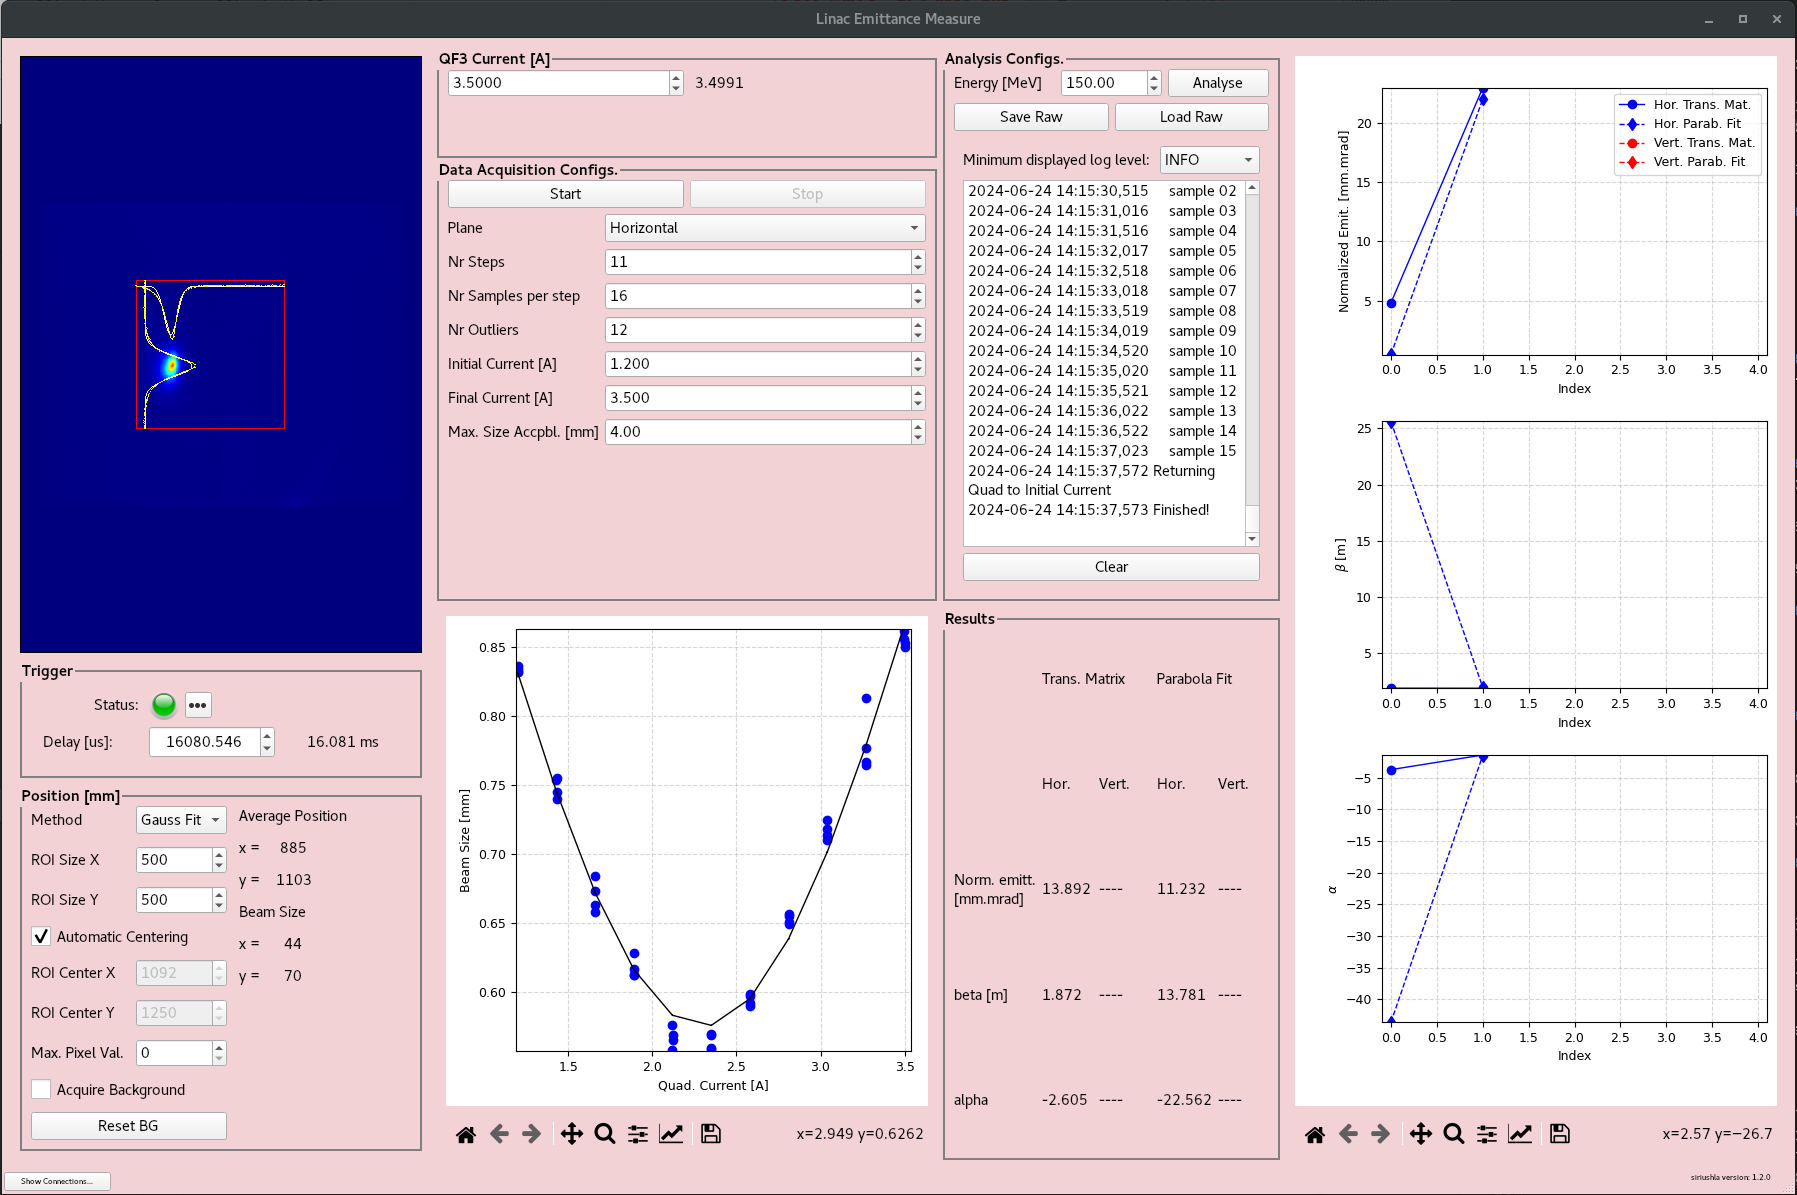
\includegraphics[width=\textwidth]{2024-07-12/figures/emitx_meas_bias_m30p4_charge_3p0nc.png}
        \caption{3 nC Horizontal Emitt.}
        \label{fig:a}
    \end{minipage}
    \hspace{0.3cm}
    \begin{minipage}[b]{0.4\linewidth}
        \centering
        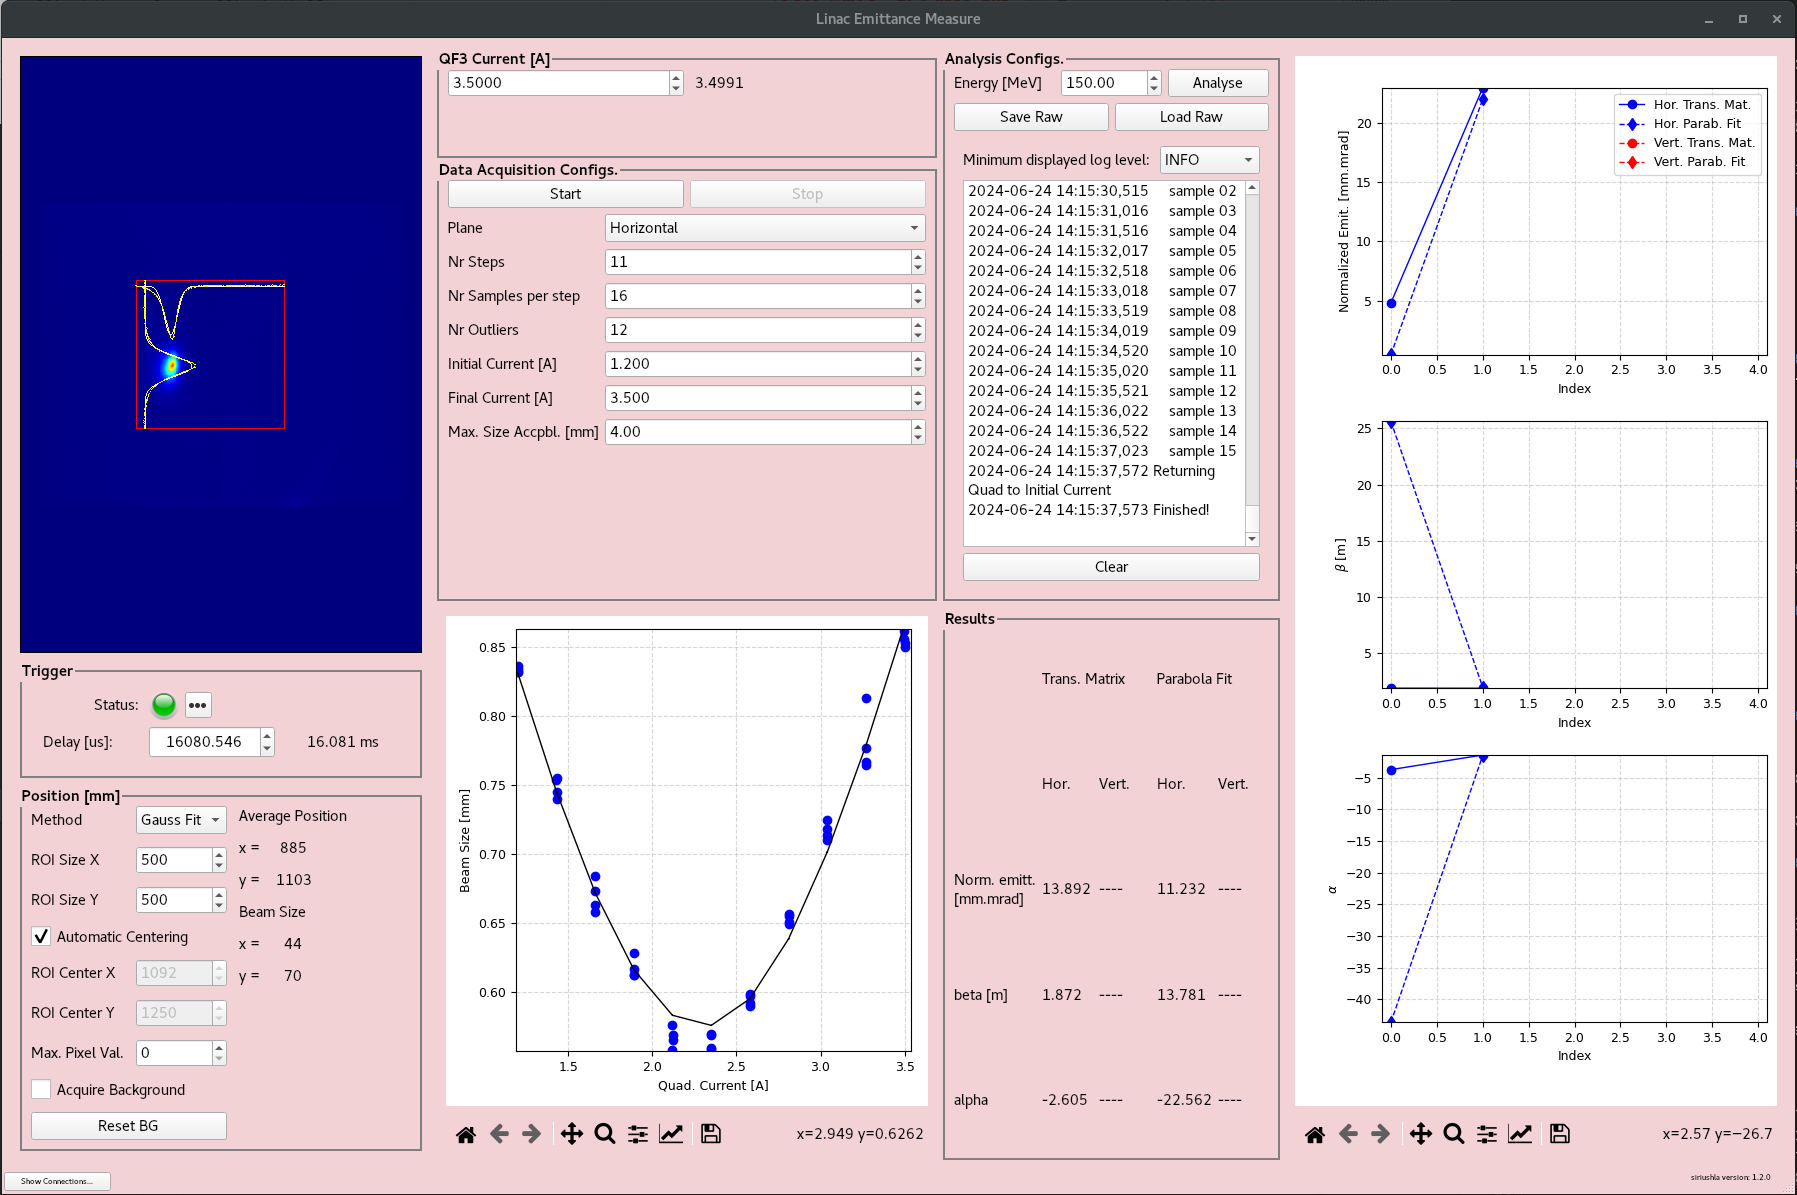
\includegraphics[width=\textwidth]{2024-07-12/figures/emitx_meas_bias_m30p4_charge_3p0nc.png}
        \caption{1.2 nC Horizontal Emitt.}
        \label{fig:b}
    \end{minipage}
\end{figure}
\end{frame}
